%! suppress = TooLargeSection
\documentclass[conference]{IEEEtran}
\usepackage{cite}
%\usepackage{amsmath,amssymb,amsfonts}
\usepackage{algorithmic}
\usepackage{graphicx}
\usepackage{textcomp}
\usepackage{xcolor}

\usepackage{subfig}
\usepackage[hidelinks]{hyperref}
\graphicspath{ {images/} }
\usepackage{pgfplots}
\pgfplotsset{compat=1.17}

\newcommand\BibTeX{{\textrm{B} \kern-.05em{\textsc{i} \kern-.025em b}\kern-.08em
T\kern-.1667em\lower.7ex\hbox{E}\ker,n-.125emX}}

\begin{document}

    \title{Clothing Item Generation using GANs}

    \author{\IEEEauthorblockN{Charlie Brayton (014559415)}
    \IEEEauthorblockA{\textit{Department of Software Engineering} \\
    \textit{San José State University}\\
    San José, California \\
    charles.brayton@sjsu.edu}
    \and
    \IEEEauthorblockN{Mohit Patel (014501461)}
    \IEEEauthorblockA{\textit{Department of Software Engineering} \\
    \textit{San José State University}\\
    San José, California \\
    mohit.patel@sjsu.edu}
    \and
    \IEEEauthorblockN{Andrew Selvia (014547273)}
    \IEEEauthorblockA{\textit{Department of Software Engineering} \\
    \textit{San José State University}\\
    San José, California \\
    andrew.selvia@sjsu.edu}
    \and
    \IEEEauthorblockN{Dylan Zhang (013073437)}
    \IEEEauthorblockA{\textit{Department of Software Engineering} \\
    \textit{San José State University}\\
    San José, California \\
    dylan.zhang@sjsu.edu}
    }

    \maketitle

    \begin{abstract}

        The primary objective of this research is to classify and generate images of clothing items.\ The work is a compilation of three distinct efforts: (1) to classify fashion-mnist images and, inversely, fool it with adversarial noise; (2) to generate novel images which emulate the true fashion-mnist images;\ (3) to infuse the grayscale images with life-like colors.\ Together, these endeavours pushed the team to explore topics at the forefront of modern machine learning, most notably generative adversarial networks (GANs).

    \end{abstract}

    \begin{IEEEkeywords}
        machine learning, computer vision, neural networks, generative adversarial networks
    \end{IEEEkeywords}

    \section{Introduction}\label{sec:introduction}

    The diverse branches of this project were made possible by the careful selection of a dataset.\ The fashion-mnist dataset was chosen specifically for its prevalence as a benchmark in recent research into neural networks.\ Its size, labels, and compatibility (with the long-established MNIST dataset) make it an ideal choice for evaluating deep neural networks (NNs) and GANs. Rather than attempt to introduce a truly groundbreaking NN architecture given the authors' limited experience, this project aims for breadth.

    Each subproject explores a unique research area with industrial applications which may answer the associated questions:

    \begin{enumerate}
        \item Classification: Can we quickly identify an item of clothing to automate sorting and retrieval?\ Supposing such an automated system existed, how susceptible might it be to failure?
        \item Generation: Can the product development lifecycle for clothing be accelerated by avoiding physical prototyping?
        \item Colorization: Can grayscale clothing imagery be augmented with colors to enable A/B testing of styles to increase customer satisfaction?
    \end{enumerate}

    To aid comprehension, each subproject is explored independently.

    \section{Data}\label{sec:data}

    The fashion-mnist dataset is composed of 60,000 training images and 10,000 testing images.\ In keeping with the legacy of the traditional MNIST, fashion-mnist images are 28x28 grayscale pixels.\ Each image is labeled as one of the ten classes enumerated below:

    \begin{enumerate}
        \setcounter{enumi}{-1}
        \item T-shirt/top
        \item Trouser
        \item Pullover
        \item Dress
        \item Coat
        \item Sandal
        \item Shirt
        \item Sneaker
        \item Bag
        \item Ankle Boot
    \end{enumerate}

    \section{Implementation}\label{sec:implementation}

    \subsection{Classification}\label{subsec:implementation-classification}
    
    Classification was performed using two neural network architectures, one using only dense layers and another using convolutional layers. The first architecture, shown in Fig~\ref{figclass1}, flattens the 28 by 28 pixel image into a vector 784 pixels long, which is then densely connected to a 128 node layer; finallly, the 128 node layer is densely connected to a 10 node output layer. The second architecture, shown in Fig~\ref{figclass2}, scans the image with a convolutional neural network using a 5 by 5 window and 64 layers; the results of the first convolutional layer are then scanned by another convolutional layer with a 5 by 5 window and 128 layers. The final step is to flatten the layer and densely connect it to the 10 node output layer. The output layer of both architectures indicates the networks confidence that the image belongs to each of the classes, so a large value in 0th node and the 6th node would indicate that the network is uncertain whether an image should be classified as a T-shirt/top or just a Shirt. The neural networks described were constructed using Keras and Tensorflow in python notebooks.
    
    The robustness of the classifier was tested by adding adversarial signals to the input images. The adversarial signal was calculated by determining the gradient of the loss function based on the input image used. This allows the adversarial signal to skew the image to the closest incorrect classification. Once the adversarial signal was determined it was scaled by an epislon value (between 0 and 1) and added to the image; for adding this noise the image is considered to be all pixels that have a brightness value greater than 0. Limiting the noise to non-zero values means the classification isn't being skewed due to noise added in the black background portions of the image. Robustness was determined by comparing the accuracy of our classifiers against ever increasing epsilon values.

    \subsection{Generation}\label{subsec:implementation-generation}

    https://github.com/AndrewSelviaSJSU/pytorch-generative-model-collections

    \subsection{Colorization}\label{subsec:implementation-colorization}
	
	The images in the fashion mnist dataset are all grayscale images. We decided to build a machine learning model that would fill colors into these black and white images intelligently. There were several techniques available to explicitly fill colors into the grayscale images. However, in order to smartly colorize the fashion mnist dataset we decided that Generative Adversarial Networks were the best choice for this task. 

	To build a model capable of smartly colorizing grayscale images we had to first build a dataset for training our GAN model. For this we combined the training and testing sets of the fashion mnist dataset. After this, we explicitly filled colors into these 70,000 grayscale images. Initially, the shape of each image was (28,28,1). After colorizing the images, their shape changed to (28,28,3). This marked the addition of 3 rows for each item in the dataset. This change happened to store the values of the red, blue and green elements of each image. Each label of the fashion mnist dataset was assigned different colors, for instance, ankle boots were colored brown and dresses were colored red. Now, we had 70,000 data instances each representing a colored fashion item from the fashion mnist dataset of the shape (28,28,3).

    
	\begin{figure}[!h]
	\begin{center}
	\caption{Training samples for colorization}
	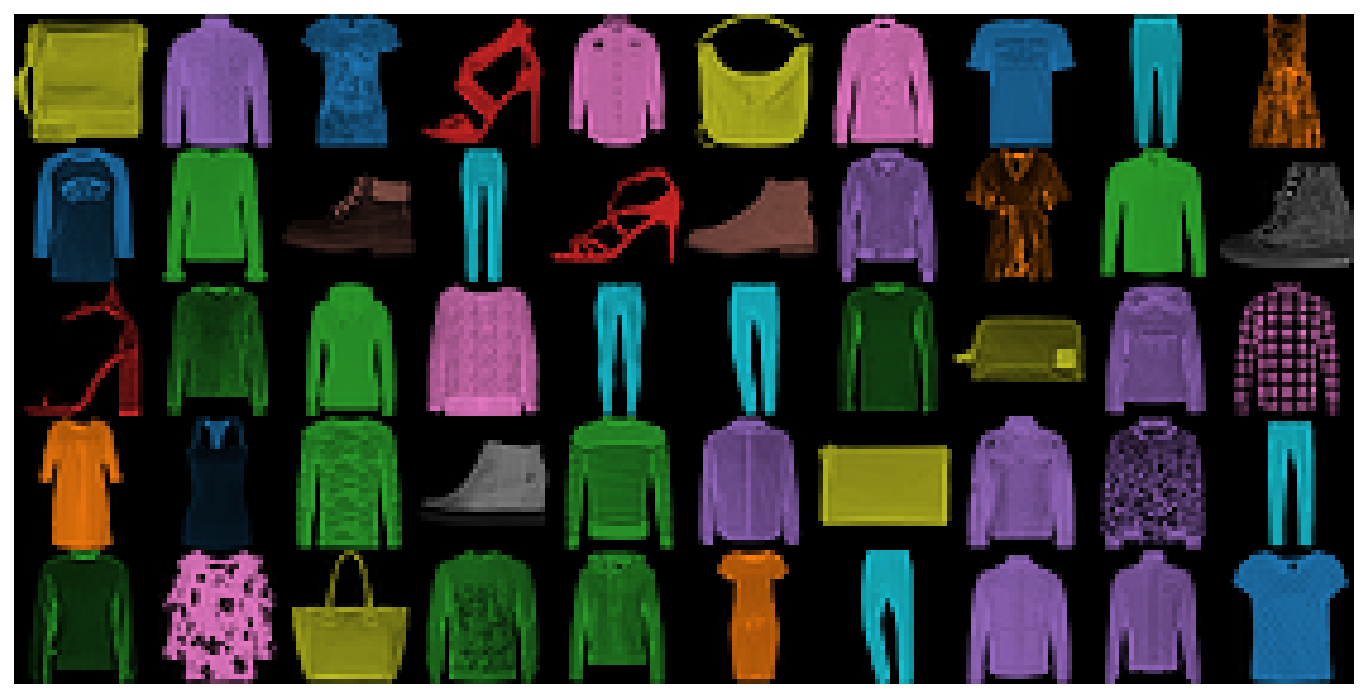
\includegraphics[scale = 0.33]{Colorization_training_samples.png}
	\end{center}
	\end{figure}

	Once we had built our training samples, we decided to work on our GAN. We fed the generator in the network the original grayscale images from the fashion mnist dataset. The generator then tried to fill colors into these grayscale images of fashion items using some randomly set weights. These generated images were then passed on to the discriminator. Along with these images, the discriminator also received the explicitly colored images from the training sample. The discriminator tried to identify which image was created from the generator and which was drawn from the training sample. Based on the decision made on the classification task by the discriminator, the discriminator loss as well as the generator loss were computed. 

	The discriminator in the network learnt from the discriminator loss by backpropagating through the discriminator node and updating the weights associated with the discriminator. Similarly, the generator updated its weights using the results obtained from backpropagating through the generator node and using the generator loss. This process of updating the weights and learning was carried out iteratively. After running this iterative process for certain epochs, we had the final weights for the network that were capable of colorizing the items in the fashion mnist dataset intelligently. 

    \section{Results}\label{sec:results}

    \subsection{Classification}\label{subsec:results-classification}
    
    

    \subsection{Generation}\label{subsec:results-generation}

    \begin{figure}
        \caption{ACGAN Learning to Generate Clothing Images}
        \label{fig:results1}
        \centering
        \subfloat[\centering Epoch 1]{{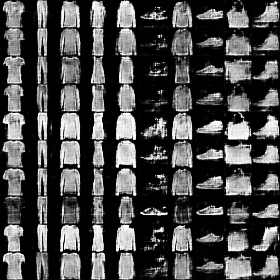
\includegraphics[width=2.5cm]{ACGAN_epoch001.png} }}
        \subfloat[\centering Epoch 25]{{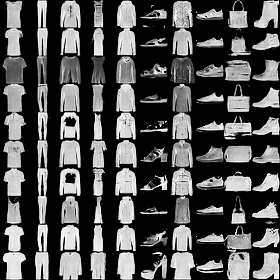
\includegraphics[width=2.5cm]{ACGAN_epoch025.png} }}
        \subfloat[\centering Epoch 50]{{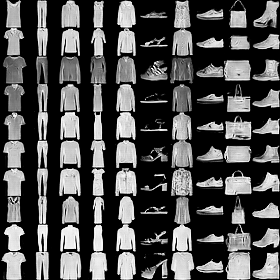
\includegraphics[width=2.5cm]{ACGAN_epoch050.png} }}
    \end{figure}

    \subsection{Colorization}\label{subsec:results-colorization}

    Here is an example of how we should cite our references~\cite{e-in-style}.

    Here is another example of citing a reference~\cite{pytorch-generative-model-collections}.

    Here is an example of how we should reference our figures~\autoref{fig:loss-and-accuracy}.

    Here is an example with multiple images~\autoref{fig:results1}

    \begin{figure}
        \caption{Loss and Accuracy}
        \label{fig:loss-and-accuracy}
        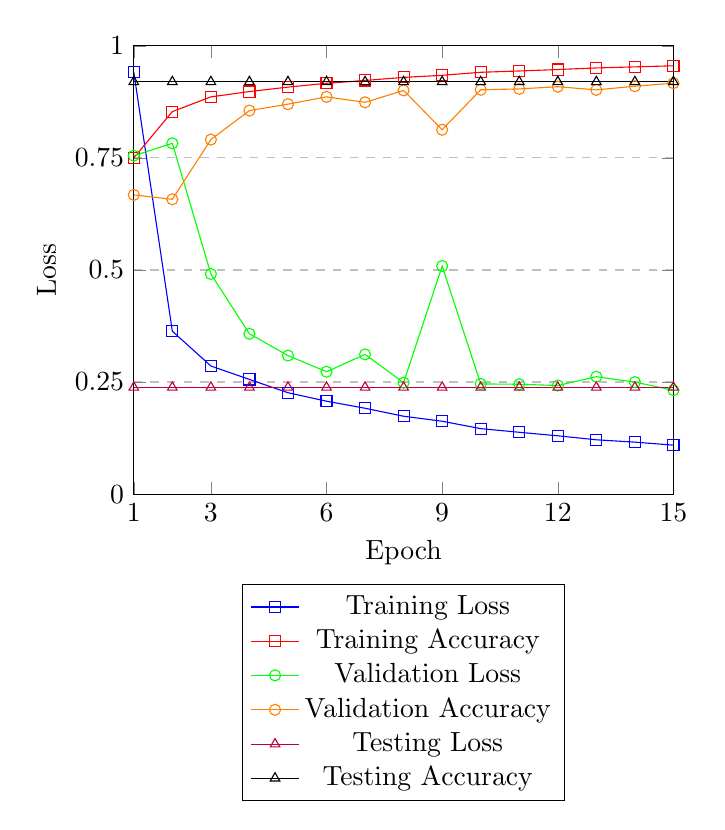
\begin{tikzpicture}
            \begin{axis}[
            xlabel={Epoch},
            ylabel={Loss},
            xmin=1, xmax=15,
            ymin=0, ymax=1,
            xtick={1, 3, 6, 9, 12, 15},
            ytick={0, .25, .50, .75, 1},
            legend style={at={(0.5,-0.2)},anchor=north},
            ymajorgrids=true,
            grid style=dashed,
            ]
                \addplot[
                color=blue,
                mark=square
                ]
                coordinates {
                (1, 0.9415369913395908)
                (2, 0.36347173816627926)
                (3, 0.2858551138391097)
                (4, 0.25580175934980315)
                (5, 0.22619957197457552)
                (6, 0.20731205224163002)
                (7, 0.19158202114825448)
                (8, 0.17376136417604154)
                (9, 0.1625804718480342)
                (10, 0.14612651362808216)
                (11, 0.1379509448694686)
                (12, 0.13010555795497364)
                (13, 0.12118976314862569)
                (14, 0.11594720014060537)
                (15, 0.10928217275068164)
                };
                \addplot[
                color=red,
                mark=square
                ]
                coordinates {
                (1, 0.7498944)
                (2, 0.8532715)
                (3, 0.8860656)
                (4, 0.8979578)
                (5, 0.90786415)
                (6, 0.9164315)
                (7, 0.9227066)
                (8, 0.9295607)
                (9, 0.9342024)
                (10, 0.94093925)
                (11, 0.94384027)
                (12, 0.9471116)
                (13, 0.9506346)
                (14, 0.9530575)
                (15, 0.9554094)
                };
                \addplot[
                color=green,
                mark=o
                ]
                coordinates {
                (1, 0.7549296505749226)
                (2, 0.7825332581996918)
                (3, 0.4910720940679312)
                (4, 0.357665928080678)
                (5, 0.3090804498642683)
                (6, 0.27299756929278374)
                (7, 0.31170774064958096)
                (8, 0.2485608123242855)
                (9, 0.508794916793704)
                (10, 0.24579987488687038)
                (11, 0.2450892459601164)
                (12, 0.24228437338024378)
                (13, 0.2619198402389884)
                (14, 0.24979994911700487)
                (15, 0.23182532005012035)
                };
                \addplot[
                color=orange,
                mark=o
                ]
                coordinates {
                (1, 0.66744876)
                (2, 0.6575944)
                (3, 0.79087156)
                (4, 0.8555428)
                (5, 0.86985517)
                (6, 0.88613117)
                (7, 0.8739339)
                (8, 0.9004858)
                (9, 0.81274575)
                (10, 0.901945)
                (11, 0.9038338)
                (12, 0.9087785)
                (13, 0.9017017)
                (14, 0.90983397)
                (15, 0.91657144)
                };
                \addplot[mark=triangle, color=purple]
                coordinates {
                (1, 0.23809038553127024)
                (2, 0.23809038553127024)
                (3, 0.23809038553127024)
                (4, 0.23809038553127024)
                (5, 0.23809038553127024)
                (6, 0.23809038553127024)
                (7, 0.23809038553127024)
                (8, 0.23809038553127024)
                (9, 0.23809038553127024)
                (10, 0.23809038553127024)
                (11, 0.23809038553127024)
                (12, 0.23809038553127024)
                (13, 0.23809038553127024)
                (14, 0.23809038553127024)
                (15, 0.23809038553127024)
                };
                \addplot[mark=triangle, color=black]
                coordinates {
                (1, 0.9196472)
                (2, 0.9196472)
                (3, 0.9196472)
                (4, 0.9196472)
                (5, 0.9196472)
                (6, 0.9196472)
                (7, 0.9196472)
                (8, 0.9196472)
                (9, 0.9196472)
                (10, 0.9196472)
                (11, 0.9196472)
                (12, 0.9196472)
                (13, 0.9196472)
                (14, 0.9196472)
                (15, 0.9196472)
                };
                \legend{Training Loss, Training Accuracy, Validation Loss, Validation Accuracy, Testing Loss, Testing Accuracy}
            \end{axis}
        \end{tikzpicture}
    \end{figure}

    \section{Conclusion}\label{sec:conclusion}

    \bibliographystyle{ieeetr}
    \bibliography{report}
\end{document}
